\section{Exact definitions of generators, procedures and estimators}\label{app:defs}
These definitions follow the code in \texttt{analysis/} (\texttt{synth.py}, \texttt{lib.py}, \texttt{run\_grid.py}); the table of scripts is in \texttt{REPRODUCE.md}. Throughout, $S\in\{0,1\}^{K\times n}$ holds the correctness of the $K$ candidates on the $n$ tuning items, $\hat p_c$ is the row mean, $\hat c$ the selected row, and ties in an argmax are broken at random.

\paragraph{Synthetic generator.} A pool of $128$ configurations and $N=20{,}000$ items. Configuration accuracies are $p_c=\mathrm{clip}(m+\tau z_c,0.01,0.99)$ with $z_c\sim N(0,1)$ ($m=0.3$ unless stated); an optional outlier raises one configuration's accuracy by a fixed amount. Each item has a latent $q_i\sim N(0,1)$ shared across configurations, and configuration $c$ has the latent $U_{ci}=\sqrt\rho\,q_i+\sqrt{1-\rho}\,e_{ci}$ with $e_{ci}\sim N(0,1)$; it is correct on item $i$ iff $U_{ci}<\Phi^{-1}(p_c)$, so every row has accuracy $p_c$ in expectation and any two rows have latent correlation $\rho$. The true accuracy $\mu_c$ of a configuration is its mean over the $N$ pool items (the pool is the population). A tuning set is $n$ items drawn with replacement; the $K$ candidates are drawn without replacement from the $128$ configurations. \emph{Generation noise} flips each evaluation of a candidate (and of the baseline) with probability $\varepsilon$ independently, and the truth becomes $\mu_c+\varepsilon(1-2\mu_c)$. \emph{Leakage}: each candidate shows $\ell$ tuning items with their answers in the prompt, which turns an incorrect outcome on such an item into a correct one with probability $0.9$; the truth is unchanged, and the held-out split scores its report half without leakage.

\paragraph{Search procedures.} \emph{Best-of-$K$}: $\hat c=\arg\max_c\hat p_c$ on all $n$ items. \emph{Successive halving}: $R=\lceil\log_2K\rceil$ rounds; the $n$ items are cut into $R$ consecutive blocks; in round $r$ the survivors are scored on block $r$ only and the better $\lceil|\text{alive}|/2\rceil$ stay; the report is the survivor's score on all $n$ items. \emph{Successive rejects}: budget $B=nK/4$ evaluations, $\bar\ell=\tfrac12+\sum_{i=2}^{K}1/i$; in phase $j=1,\dots,K-1$ the survivors are scored on the first $n_j=\min\{n,\max\{1,\lceil (B-K)/(\bar\ell(K+1-j))\rceil\}\}$ items and the worst is removed; the report is the winner's mean over the first $n_{K-1}$ items. \emph{Greedy coordinate ascent}: the $K$ candidates form a factorial grid ($4\times4\times4$, or $8\times4\times4$ for $K=128$); start at a random cell and, for the factors in random order, move to the best level given the others on all $n$ items, for at most $10$ sweeps; the report is the final cell's score.

\paragraph{Claim test and baseline.} The baseline is pool configuration $0$, scored on the same $n$ items as the candidates (on the report items for the held-out split), with the same generation noise. For any method with point report $\hat\theta$ and critical value $z$ ($1.645$; the simultaneous critical value $c$ for the simultaneous bound), the claim is $(\hat\theta-\hat p_{\text{base}})/\mathrm{dse}>z$, where $\mathrm{dse}$ is the standard deviation (ddof 1) of the per-item differences $S_{\hat c,i}-S_{\text{base},i}$ divided by $\sqrt{n_{\text{rep}}}$ ($n_{\text{rep}}$ the number of report items). The false-claim rate is the mean of the claim indicator over repetitions with $\mu_{\hat c}\le\mu_{\text{base}}$. A false ship is $\hat\theta\ge\mu_{\text{base}}+0.02$ and $\mu_{\hat c}<\mu_{\text{base}}+0.02$.

\paragraph{Reporting methods.} All intervals are $95\%$ ($\alpha=0.05$) and Wilson intervals use the number of items the report was computed from.
\emph{Naive}: $\hat p_{\hat c}$ with a Wilson interval on $n$. \emph{Held-out split}: the search runs on the first $\lfloor n/2\rceil$ items (the tuning set is in random order), the report is the pick's mean on the remaining items with a Wilson interval on their number. \emph{Five-fold cross-fitting}: $n$ items in five consecutive folds; for each fold the procedure runs on the other four and its pick is scored on the fold; the report is the pooled score over all $n$ items, with a Wilson interval on $n$; the configuration it describes is the full-data pick. \emph{Bootstrap}: $B=100$ resamples of the $n$ items with replacement; for each, the procedure is run on the resample, giving pick $\hat c_b$; the optimism is the score of $\hat c_b$ on the resample minus its score on the original items, and the optimism-corrected report is the naive score minus the mean optimism; the out-of-bag report is the mean score of $\hat c_b$ on the items absent from resample $b$; the $.632$ report is $0.368\,\hat p_{\hat c}+0.632\,\text{OOB}$; intervals are the report $\pm1.96\sqrt{\hat\theta(1-\hat\theta)/n}$, i.e.\ they ignore the selection. \emph{Simultaneous bound}: $B=300$ bootstrap resamples of the items; $c$ is the $0.95$ quantile of $\max_k|\hat p^*_k-\hat p_k|/\mathrm{se}_k$ with $\mathrm{se}_k=\sqrt{\max(\hat p_k(1-\hat p_k),10^{-4})/n}$; the interval is $\hat p_{\hat c}\pm c\,\mathrm{se}_{\hat c}$ and the point report is naive. \emph{Ladder}: $\eta=1/\sqrt n$; candidates are visited in a random order; the first sets the ladder value $\mathrm{round}(\hat p/\eta)\eta$, a later one replaces the selected configuration and the value only if $\hat p>\text{value}+\eta$; the report is the final value with a Wilson interval on $n$.

\paragraph{Conditional and hybrid intervals.} Both treat $\hat p\sim N(\mu,\hat\Sigma/n)$ with $\hat\Sigma$ the sample covariance of the rows of $S$, and apply to best-of-$K$ only. To remove lattice ties each score is dithered by one uniform draw on $\pm1/(2n)$ per repetition, used for every quantity of that repetition, which leaves the argmax a random-tie argmax. Given the winner $\hat c=k$, the event $\{\hat c=k\}$ is a polyhedron in $\hat p_k$ once the component of $\hat p$ orthogonal to $\hat p_k$ is fixed (the polyhedral lemma of \citet{lee2016exact}, in the form for the winner of a maximum \citep{andrews2024winners}); its truncation interval $[V^-,V^+]$ is computed from the $K-1$ contrasts. \emph{Conditional}: the conditional law of $\hat p_k$ is $N(\theta,\sigma_k^2)$ truncated to $[V^-,V^+]$; the estimate is the $\theta$ at which the conditional CDF at the observed value equals $1/2$ and the interval endpoints are the $\theta$ at which it equals $1-\alpha/2$ and $\alpha/2$ (root-finding on $\hat p_k\pm80\sigma_k$). \emph{Hybrid}: $\beta=0.005$; $c_\beta$ is the $1-\beta$ quantile (from $1000$ Monte-Carlo draws) of $\max_j|Z_j|$ with $Z\sim N(0,\text{corr}(\hat\Sigma))$; for each $\theta_0$ on a grid of $161$ values in $\hat p_k\pm c_\beta\sigma_k$ the truncation interval is intersected with $[\theta_0-c_\beta\sigma_k,\theta_0+c_\beta\sigma_k]$, and $\theta_0$ is retained if the conditional CDF of $\hat p_k$ lies in $[a_1,1-a_1]$ with $a_1=(\alpha-\beta)/(2(1-\beta))$; the interval is the range of retained values and the point estimate is the median of the truncated normal on the restricted set (the hybrid median-unbiased estimate, always within $\hat p_k\pm c_\beta\sigma_k$). The conditional point estimate is the unrestricted conditional median.
\emph{Validation.} (1) For $K=2$ the conditional CDF equals an independent closed form (computed with mpmath) to $\N{val_k2_cdf}$ over $2000$ draws. (2) With exact Gaussian draws and known $\Sigma$ ($\N{val_ncases}$ cases, $K=2$--$16$, $\tau$ from $0$ to $.05$, $n$ from $200$ to $1000$, $3000$ repetitions) the probability-integral transform of the conditional CDF at the true score is uniform (Kolmogorov--Smirnov $p$-values $\N{val_ks_min}$--$\N{val_ks_max}$) and both intervals cover $\N{val_cov_min}$--$\N{val_cov_max}\%$. (3) A Python port of the authors' MATLAB replication code for the conditional and hybrid routines agrees on $\N{val_akm_n}$ random covariance matrices ($\N{val_akm_skip}$ more were skipped because the port's truncated-normal quantile saturates): truncation limits to $10^{-12}$, conditional limits and median to about $10^{-6}$ standard errors, hybrid limits to within one step of our $161$-point grid (the port uses $4001$ points) and the hybrid median to $0.04$ of a step. (4) In the reference cell with known $\Sigma$ the conditional interval covers $\N{val_ref_cond_cov_known}\%$ (with $\Sigma$ estimated from Bernoulli draws: $\N{val_ref_cond_cov_est}\%$), with mean width $\N{val_ref_cond_width_mean}$ and median width $\N{val_ref_cond_width_med}$~pp.

\paragraph{Real replay.} The correctness matrix $Y\in\{0,1\}^{K\times2000}$ is fixed. Each repetition draws $n$ items without replacement as the tuning set (candidates are all $K$ complete configurations, or a random subset), runs a procedure and a reporting method on them, and takes as truth the selected configuration's accuracy on the other $2000-n$ items. The baseline for claims is the hand-written default (instruction $0$, demonstration set $1$, plain layout; accuracy $19.15\%$), which is one of the candidates when all $K$ are searched. Greedy coordinate search is run on the $6\times5\times2$ grid of instruction, demonstration set and layout (all $60$ configurations), with the same random start and sweeps as in the synthetic study. In the i.i.d. arm the $n$ items are drawn with replacement and the truth is the accuracy of the selected configuration on all $2000$ items. The Gaussian-maximum prediction for the real matrix uses $\epsilon\sim\mathcal N(0,\hat\Sigma/n)$ with $\hat\Sigma$ the empirical covariance of the $0/1$ item matrix of the $K$ candidates ($5000$ draws). In the disjoint arm the truth is the accuracy on the $N-n$ remaining items ($N=2000$), so the tuning noise has covariance $(1-n/N)\hat\Sigma/n$ and the predicted gap is $N/(N-n)$ times the expected noise of the selected configuration. The generator matched to the real matrix (Appendix~\ref{app:calib}) uses the real accuracies as thresholds of a Gaussian copula with either one latent correlation or the pairwise tetrachoric correlation matrix of the real $0/1$ data (eigenvalues clipped to be positive semi-definite)..

\section{Further reporting-method results}\label{app:more}
The other methods mostly fail the criterion, for different reasons. The naive report fails in all but $\N{rel_naive_ok}$ of $106$ cells, under-covering in $\N{rel_naive_under}$. The simultaneous bound keeps the naive bias ($\N{ref_simul_bias}$~pp) but under-covers in only $\N{rel_simul_under}$ cells and over-covers in $\N{rel_simul_over}$ ($\N{ref_simul_cover}\%$ in the reference cell), at a width of $\N{ref_simul_width}$~pp: it is valid and conservative. Five-fold cross-fitting has bias near zero in $\N{rel_crossfit_okb}$ cells but under-covers in $\N{rel_crossfit_under}$ ($\N{ref_crossfit_cover}\%$ in the reference cell) because its interval ignores the variance added by selection. The bootstrap optimism correction reduces the bias from $\N{ref_naive_bias}$ to $\N{ref_boot_opt_bias}$~pp and its out-of-bag variant to $\N{ref_boot_oob_bias}$~pp (bias criterion met in $\N{rel_boot_oob_okb}$ cells) but over-covers in $\N{rel_boot_oob_over}$ cells ($\N{ref_boot_oob_cover}\%$ in the reference cell) and under-covers in $\N{rel_boot_oob_under}$, so it meets the full criterion in only $\N{rel_boot_oob_ok}$ of $106$. Our implementation of winner-aware conditional inference was run in $\N{rel_cond_cells}$ cells; it covers correctly in the reference cell ($\N{ref_cond_cover}\%$) and is outside the band in $\N{rel_cond_under}$ (under) and $\N{rel_cond_over}$ (over) of them, but its intervals are very wide ($\N{ref_cond_width}$~pp), its heavy-tailed conditional median has RMSE $\N{ref_cond_rmse}$~pp and it meets the bias criterion in $\N{rel_cond_okb}$ of them. The instability is not a coding fault (Appendix~\ref{app:defs}): the conditional median is median-unbiased, but when the winner's standardised lead over the truncation boundary is small the truncated normal is nearly flat over a long left tail in the score, so the mean error is large. In the reference cell with known $\Sigma$ the lead is below $0.5$ standard errors in $\N{val_ref_lead_lt05}\%$ of repetitions (median $\N{val_ref_lead_med}$); in the $\N{lead_ref_share_small}\%$ with a lead below $0.25$ the conditional median has median error $\N{lead_ref_condmed_err}$~pp and mean error $\N{lead_ref_condmean_err}$~pp and its interval has median width $\N{lead_ref_condwidth_med}$~pp, while the hybrid has mean error $\N{lead_ref_hyberr}$~pp at width $\N{lead_ref_hybwidth}$~pp. Over all repetitions the point-estimate RMSE is $\N{val_ref_cond_rmse}$~pp for the conditional and $\N{val_ref_hyb_rmse}$~pp for the hybrid median (median absolute error $\N{val_ref_cond_medae}$ and $\N{val_ref_hyb_medae}$~pp). With one clearly better configuration ($+5$~pp, $K=16$, $n=500$) the winner is the truly best in $\N{lead_clear_n500_best}\%$ of repetitions ($\N{lead_clear_n1000_best}\%$ at $n=1000$, where the conditional interval is $\N{lead_clear_n1000_width}$~pp wide, as wide as the naive one). The conditional interval is thus a correct but uninformative answer when the data barely separate the winner from the rest. A hybrid interval of the same family (projection interval plus the conditional test on the restricted truncation set) has coverage $\N{hy_hybrid_covmin}$--$\N{hy_hybrid_covmax}\%$ at a mean width of $\N{hy_hybrid_width}$~pp over $\N{hy_cells}$ cells of the $\tau\times n\times K$ grid ($\N{hy_reps}$ repetitions each; Fig.~\ref{fig:hybrid} in Appendix~\ref{app:figs}), against $\N{hy_naive_covmin}$--$\N{hy_naive_covmax}\%$ at $\N{hy_naive_width}$~pp for the naive interval and $\N{hy_simul_covmin}$--$\N{hy_simul_covmax}\%$ at $\N{hy_simul_width}$~pp for the simultaneous bound. It needs the full-evaluation argmax and a Gaussian approximation and was checked only at $\rho=0.5$, mean accuracy $0.3$ and $K\le64$; we do not recommend it for its point estimate. The Ladder-type report \citep{blum2015ladder} (sequential submission) reduces the naive bias but does not remove it ($\tau=0$, $n=200$, $K=16$: $\N{lad_ladder_K16_bias}$ vs.\ $\N{lad_naive_K16_bias}$~pp).

\begin{table}[h]
\centering
\caption{Reporting methods in the reference cell, exact truth. Every row is scored against the true accuracy of the configuration it reports on: the selected configuration for all rows except the held-out split, which reports on the configuration chosen from $n/2$ items (Table~\ref{tab:fresh} compares protocols at equal total items).}\label{tab:ref}
{\footnotesize\setlength{\tabcolsep}{3.5pt}
\begin{tabular}{lrrrrrr}
\toprule
method & bias (pp) & RMSE (pp) & coverage & width (pp) & false claim & false ship \\
\midrule
naive (same items) & $4.59 \pm 0.06$ & 5.25 & $0.759 \pm 0.010$ & 13.1 & 0.248 & 0.818 \\
held-out split & $0.07 \pm 0.11$ & 4.72 & $0.946 \pm 0.005$ & 17.6 & 0.036 & 0.327 \\
5-fold cross-fit & $0.00 \pm 0.09$ & 4.23 & $0.866 \pm 0.008$ & 12.6 & 0.070 & 0.278 \\
bootstrap optimism & $1.27 \pm 0.06$ & 3.14 & $0.966 \pm 0.004$ & 13.2 & 0.051 & 0.356 \\
bootstrap out-of-bag & $-0.09 \pm 0.06$ & 2.86 & $0.974 \pm 0.004$ & 12.7 & 0.017 & 0.207 \\
bootstrap .632 & $1.63 \pm 0.06$ & 3.18 & $0.960 \pm 0.004$ & 12.9 & 0.058 & 0.411 \\
simultaneous bound & $4.57 \pm 0.06$ & 5.25 & $0.983 \pm 0.003$ & 19.4 & 0.012 & 0.818 \\
conditional (winner-aware) & $-10.45 \pm 0.87$ & 40.45 & $0.952 \pm 0.005$ & 60.5 & 0.091 & 0.354 \\
\bottomrule
\end{tabular}}

\par\smallskip\begin{minipage}{.97\linewidth}\footnotesizeReference cell: n=200, K=16, $\tau$=.01, $\rho$=.5, mean accuracy .3, best-of-K; 2000 repetitions. Bias and coverage are mean $\pm$ Monte Carlo s.e.; coverage is of the nominal 95\% interval for the true score of the selected configuration; false claim: rate of claiming tuned $>$ baseline when it is not truly better; false ship: rate of reporting a score at least 2 pp above the baseline's true score while the selected configuration's true score is below that bar.
\end{minipage}
\end{table}

\begin{table}[h]
\centering
\caption{Reporting protocols at equal total items, each scored against its own shipped configuration (reference cell).}\label{tab:fresh}
{\footnotesize\setlength{\tabcolsep}{3.5pt}
\begin{tabular}{lrrrrrr}
\toprule
protocol & items & true acc. (\%) & bias (pp) & RMSE (pp) & coverage & width (pp) \\
\midrule
naive & 200 & 30.44 & $4.53 \pm 0.10$ & 5.19 & $0.762 \pm 0.017$ & 13.1 \\
bootstrap out-of-bag & 200 & 30.46 & $-0.12 \pm 0.12$ & 2.85 & $0.975 \pm 0.006$ & 12.7 \\
bootstrap optimism & 200 & 30.46 & $1.23 \pm 0.12$ & 3.13 & $0.958 \pm 0.008$ & 13.2 \\
simultaneous bound & 200 & 30.45 & $4.51 \pm 0.10$ & 5.18 & $0.970 \pm 0.007$ & 19.4 \\
5-fold cross-fit & 200 & 30.48 & $-0.04 \pm 0.18$ & 4.42 & $0.848 \pm 0.015$ & 12.6 \\
hybrid (proj.+cond.) & 200 & 30.44 & $-0.88 \pm 0.23$ & 5.63 & $0.940 \pm 0.010$ & 16.5 \\
held-out split 50/50 & 200 & 30.29 & $-0.02 \pm 0.19$ & 4.57 & $0.952 \pm 0.009$ & 17.6 \\
fresh set 50/150 & 200 & 30.20 & $-0.04 \pm 0.16$ & 3.87 & $0.940 \pm 0.010$ & 14.5 \\
fresh set 100/100 & 200 & 30.34 & $-0.23 \pm 0.18$ & 4.53 & $0.952 \pm 0.009$ & 17.6 \\
\midrule
naive & 400 & 30.59 & $3.16 \pm 0.08$ & 3.66 & $0.788 \pm 0.017$ & 9.2 \\
bootstrap out-of-bag & 400 & 30.57 & $-0.06 \pm 0.08$ & 2.07 & $0.973 \pm 0.007$ & 9.0 \\
bootstrap optimism & 400 & 30.57 & $0.91 \pm 0.08$ & 2.26 & $0.962 \pm 0.008$ & 9.3 \\
simultaneous bound & 400 & 30.57 & $3.18 \pm 0.07$ & 3.67 & $0.978 \pm 0.006$ & 13.7 \\
5-fold cross-fit & 400 & 30.57 & $0.14 \pm 0.12$ & 2.98 & $0.862 \pm 0.014$ & 9.0 \\
hybrid (proj.+cond.) & 400 & 30.58 & $-0.36 \pm 0.16$ & 4.00 & $0.950 \pm 0.009$ & 11.5 \\
held-out split 50/50 & 400 & 30.42 & $0.17 \pm 0.14$ & 3.34 & $0.928 \pm 0.011$ & 12.6 \\
fresh set 100/300 & 400 & 30.30 & $0.16 \pm 0.10$ & 2.54 & $0.950 \pm 0.009$ & 10.3 \\
fresh set 200/200 & 400 & 30.46 & $0.26 \pm 0.12$ & 2.99 & $0.960 \pm 0.008$ & 12.7 \\
\bottomrule
\end{tabular}}

\par\smallskip\begin{minipage}{.97\linewidth}\footnotesizeReference cell ($\tau$=.01, $K$=16, $\rho$=.5, mean accuracy .3, best-of-$K$), 600 repetitions; the budget (items) is the total number of questions consumed: methods above the fresh-set rows tune and report on the same items (in-sample), a fresh-set row ``$n_{\rm tune}/m$'' tunes on $n_{\rm tune}$ items and reports the winner on $m$ new items (Wilson interval). Each row is scored against its own truth, the true accuracy of the configuration that protocol shipped (third column; it differs across protocols because the search saw different data). Bias and coverage are mean $\pm$ Monte Carlo s.e.; coverage is of the nominal 95\% interval; the held-out split tunes on one half of the items and reports on the other.
\end{minipage}
\end{table}

\begin{table}[h]
\centering
\caption{Reporting methods in the real setting (best-of-$K$ with $K=\N{real_K}$ complete configurations, disjoint truth).}\label{tab:real}
{\footnotesize\setlength{\tabcolsep}{3.5pt}
\begin{tabular}{rlrrrr}
\toprule
$n$ & method & bias (pp) & RMSE (pp) & coverage & width (pp) \\
\midrule
50 & naive (same items) & $9.25 \pm 0.13$ & 10.19 & $0.641 \pm 0.015$ & 24.0 \\
 & held-out split & $-0.15 \pm 0.24$ & 7.57 & $0.960 \pm 0.006$ & 28.6 \\
 & 5-fold cross-fit & $0.17 \pm 0.21$ & 6.73 & $0.896 \pm 0.010$ & 20.8 \\
 & bootstrap optimism & $2.56 \pm 0.15$ & 5.40 & $0.985 \pm 0.004$ & 24.7 \\
 & bootstrap out-of-bag & $-0.17 \pm 0.14$ & 4.50 & $0.978 \pm 0.005$ & 21.2 \\
 & bootstrap .632 & $3.30 \pm 0.14$ & 5.48 & $0.978 \pm 0.005$ & 22.7 \\
 & simultaneous bound & $9.27 \pm 0.13$ & 10.20 & $0.995 \pm 0.002$ & 38.6 \\
 & conditional (winner-aware) & $-25.69 \pm 2.64$ & 87.26 & $0.964 \pm 0.006$ & 130.4 \\
 & hybrid (proj.+cond.) & $-1.51 \pm 0.32$ & 10.20 & $0.971 \pm 0.005$ & 32.4 \\
\midrule
200 & naive (same items) & $4.18 \pm 0.07$ & 4.80 & $0.709 \pm 0.014$ & 11.6 \\
 & held-out split & $-0.07 \pm 0.13$ & 4.00 & $0.944 \pm 0.007$ & 15.0 \\
 & 5-fold cross-fit & $-0.09 \pm 0.12$ & 3.76 & $0.843 \pm 0.012$ & 10.7 \\
 & bootstrap optimism & $0.97 \pm 0.08$ & 2.80 & $0.964 \pm 0.006$ & 11.6 \\
 & bootstrap out-of-bag & $-0.32 \pm 0.08$ & 2.61 & $0.966 \pm 0.006$ & 10.7 \\
 & bootstrap .632 & $1.34 \pm 0.08$ & 2.83 & $0.952 \pm 0.007$ & 11.1 \\
 & simultaneous bound & $4.17 \pm 0.08$ & 4.80 & $0.988 \pm 0.003$ & 18.4 \\
 & conditional (winner-aware) & $-11.04 \pm 1.23$ & 40.50 & $0.953 \pm 0.007$ & 56.2 \\
 & hybrid (proj.+cond.) & $-0.85 \pm 0.16$ & 5.19 & $0.966 \pm 0.006$ & 15.3 \\
\bottomrule
\end{tabular}}

\par\smallskip\begin{minipage}{.97\linewidth}\footnotesizeReal-LLM replay on MMLU-Pro with Qwen2.5-0.5B-Instruct: best-of-$K$ over the $K$=60 configurations, tuning set of $n$ questions drawn without replacement from the 2000-question pool; 1000 repetitions per row. Truth = accuracy of the selected configuration on the pool questions outside the tuning set (finite-pool truth). Bias and coverage are mean $\pm$ Monte Carlo s.e.; coverage is of the nominal 95\% interval. The bias and RMSE of the conditional method are dominated by the heavy tail of its estimate (reported as measured).
\end{minipage}
\end{table}

\begin{table}[h]
\centering
\caption{Reporting protocols at equal total items on the real matrix, each scored against its own shipped configuration.}\label{tab:freshreal}
{\footnotesize\setlength{\tabcolsep}{3.5pt}
\begin{tabular}{lrrrrrr}
\toprule
protocol & items & true acc. (\%) & bias (pp) & RMSE (pp) & coverage & width (pp) \\
\midrule
naive & 200 & 18.82 & $4.46 \pm 0.11$ & 5.10 & $0.650 \pm 0.021$ & 11.6 \\
bootstrap out-of-bag & 200 & 18.81 & $-0.05 \pm 0.12$ & 2.74 & $0.944 \pm 0.010$ & 10.8 \\
bootstrap optimism & 200 & 18.81 & $1.23 \pm 0.12$ & 3.00 & $0.956 \pm 0.009$ & 11.7 \\
simultaneous bound & 200 & 18.83 & $4.45 \pm 0.11$ & 5.09 & $0.986 \pm 0.005$ & 18.4 \\
5-fold cross-fit & 200 & 18.81 & $0.08 \pm 0.16$ & 3.65 & $0.856 \pm 0.016$ & 10.7 \\
hybrid (proj.+cond.) & 200 & 18.82 & $-0.46 \pm 0.22$ & 4.99 & $0.966 \pm 0.008$ & 15.4 \\
held-out split 50/50 & 200 & 18.54 & $0.08 \pm 0.18$ & 3.91 & $0.948 \pm 0.010$ & 15.0 \\
fresh set 50/150 & 200 & 18.46 & $-0.04 \pm 0.15$ & 3.36 & $0.936 \pm 0.011$ & 12.3 \\
fresh set 100/100 & 200 & 18.58 & $0.05 \pm 0.17$ & 3.76 & $0.950 \pm 0.010$ & 15.0 \\
\bottomrule
\end{tabular}}

\par\smallskip\begin{minipage}{.97\linewidth}\footnotesizeReal-LLM replay on MMLU-Pro (Qwen2.5-0.5B-Instruct), best-of-$K$ with $K$=60 configurations (largest $K$ in the file), total budget 200 questions, 500 repetitions. Questions are drawn without replacement from the 2000-question pool; each row is scored against the accuracy of the configuration it shipped on the pool questions that protocol did not use (third column, true accuracy of the shipped configuration). Columns as in the synthetic table.
\end{minipage}
\end{table}

\section{Additional synthetic results}\label{app:tables}
\begin{table}[h]
\centering
\caption{Naive optimism gap by tuning-set size and number of candidates.}\label{tab:gapnk}
{\footnotesize\setlength{\tabcolsep}{3.5pt}
\begin{tabular}{rrrrr}
\toprule
$\tau$ & $n$ & $K$=4 & $K$=16 & $K$=64 \\
\midrule
0 & 100 & $3.92 \pm 0.17$ & $6.96 \pm 0.16$ & $9.14 \pm 0.14$ \\
0 & 200 & $2.90 \pm 0.12$ & $4.81 \pm 0.10$ & $6.32 \pm 0.10$ \\
0 & 500 & $1.65 \pm 0.08$ & $2.97 \pm 0.07$ & $3.98 \pm 0.07$ \\
0 & 1000 & $1.22 \pm 0.05$ & $2.04 \pm 0.05$ & $2.80 \pm 0.05$ \\
\midrule
0.03 & 100 & $3.13 \pm 0.18$ & $5.44 \pm 0.16$ & $7.44 \pm 0.16$ \\
0.03 & 200 & $2.12 \pm 0.13$ & $3.72 \pm 0.12$ & $4.58 \pm 0.13$ \\
0.03 & 500 & $0.90 \pm 0.08$ & $1.70 \pm 0.09$ & $2.18 \pm 0.09$ \\
0.03 & 1000 & $0.40 \pm 0.06$ & $0.93 \pm 0.06$ & $0.92 \pm 0.06$ \\
\bottomrule
\end{tabular}}

\par\smallskip\begin{minipage}{.97\linewidth}\footnotesizeNaive optimism gap (pp; reported minus true score of the selected configuration), mean $\pm$ Monte Carlo s.e. over 500 repetitions; $\rho$=.5, best-of-K.
\end{minipage}
\end{table}
\begin{table}[h]
\centering
\caption{Stress cells.}\label{tab:stress}
{\footnotesize\setlength{\tabcolsep}{3.5pt}
\begin{tabular}{llrrrr}
\toprule
cell & method & bias (pp) & coverage & width (pp) & false claim \\
\midrule
$n$=50, $K$=128, acc. 0.1 & naive (same items) & $10.41 \pm 0.08$ & $0.330 \pm 0.011$ & 21.9 & 0.550 \\
 & held-out split & $0.15 \pm 0.13$ & $0.967 \pm 0.004$ & 23.7 & 0.056 \\
 & 5-fold cross-fit & $0.07 \pm 0.13$ & $0.908 \pm 0.006$ & 16.5 & 0.060 \\
 & bootstrap out-of-bag & $0.04 \pm 0.07$ & $0.990 \pm 0.002$ & 16.5 & 0.004 \\
 & simultaneous bound & $10.40 \pm 0.08$ & $0.999 \pm 0.001$ & 41.9 & 0.000 \\
 & conditional (winner-aware) & $-28.54 \pm 1.83$ & $0.965 \pm 0.004$ & 138.5 & 0.117 \\
\midrule
$n$=200, $K$=16, outl. 0.03 & naive (same items) & $4.74 \pm 0.05$ & $0.757 \pm 0.010$ & 13.1 & 0.257 \\
 & held-out split & $-0.09 \pm 0.10$ & $0.949 \pm 0.005$ & 17.6 & 0.042 \\
 & 5-fold cross-fit & $0.08 \pm 0.09$ & $0.867 \pm 0.008$ & 12.6 & 0.085 \\
 & bootstrap out-of-bag & $0.01 \pm 0.06$ & $0.975 \pm 0.003$ & 12.7 & 0.025 \\
 & simultaneous bound & $4.74 \pm 0.06$ & $0.973 \pm 0.004$ & 19.4 & 0.015 \\
 & conditional (winner-aware) & $-10.23 \pm 0.83$ & $0.950 \pm 0.005$ & 62.3 & 0.104 \\
\midrule
$n$=200, $K$=128, outl. 0.03 & naive (same items) & $6.88 \pm 0.05$ & $0.409 \pm 0.011$ & 13.3 & 0.535 \\
 & held-out split & $-0.04 \pm 0.10$ & $0.953 \pm 0.005$ & 17.6 & 0.034 \\
 & 5-fold cross-fit & $-0.02 \pm 0.09$ & $0.875 \pm 0.007$ & 12.6 & 0.082 \\
 & bootstrap out-of-bag & $-0.13 \pm 0.06$ & $0.988 \pm 0.002$ & 12.7 & 0.016 \\
 & simultaneous bound & $6.87 \pm 0.05$ & $0.986 \pm 0.003$ & 23.5 & 0.014 \\
 & conditional (winner-aware) & $-13.07 \pm 0.97$ & $0.957 \pm 0.005$ & 77.5 & 0.150 \\
\midrule
$n$=200, $K$=16, outl. 0.05 & naive (same items) & $4.59 \pm 0.06$ & $0.767 \pm 0.009$ & 13.1 & 0.252 \\
 & held-out split & $-0.01 \pm 0.10$ & $0.955 \pm 0.005$ & 17.6 & 0.042 \\
 & 5-fold cross-fit & $0.02 \pm 0.09$ & $0.875 \pm 0.007$ & 12.6 & 0.082 \\
 & bootstrap out-of-bag & $-0.14 \pm 0.06$ & $0.975 \pm 0.003$ & 12.7 & 0.022 \\
 & simultaneous bound & $4.58 \pm 0.06$ & $0.983 \pm 0.003$ & 19.4 & 0.015 \\
 & conditional (winner-aware) & $-9.78 \pm 0.82$ & $0.966 \pm 0.004$ & 61.0 & 0.094 \\
\midrule
$n$=200, $K$=128, outl. 0.05 & naive (same items) & $6.10 \pm 0.07$ & $0.505 \pm 0.011$ & 13.3 & 0.546 \\
 & held-out split & $0.08 \pm 0.10$ & $0.951 \pm 0.005$ & 17.7 & 0.041 \\
 & 5-fold cross-fit & $-0.31 \pm 0.10$ & $0.846 \pm 0.008$ & 12.7 & 0.082 \\
 & bootstrap out-of-bag & $-0.76 \pm 0.07$ & $0.939 \pm 0.005$ & 12.8 & 0.017 \\
 & simultaneous bound & $6.08 \pm 0.07$ & $0.981 \pm 0.003$ & 23.6 & 0.014 \\
 & conditional (winner-aware) & $-13.77 \pm 1.04$ & $0.953 \pm 0.005$ & 72.8 & 0.152 \\
\bottomrule
\end{tabular}}

\par\smallskip\begin{minipage}{.97\linewidth}\footnotesizeStress cells ($\tau$=0, $\rho$=.5, best-of-K; outlier = fraction of outlier configurations); 2000 repetitions each. Columns as in the reference-cell table (RMSE and false-ship rate omitted for width; they are in the results file); bias and coverage are mean $\pm$ Monte Carlo s.e.; outl. = outlier-configuration fraction, acc. = mean accuracy (.3 unless shown).
\end{minipage}
\end{table}
\begin{table}[h]
\centering
\caption{Two tuned systems with unequal search budgets.}\label{tab:unequal}
{\footnotesize\setlength{\tabcolsep}{3.5pt}
\begin{tabular}{rlrrrrrr}
\toprule
$\tau$ & $K_A/K_B$ & claim (naive) & false claim & wrong sign & reported diff. (pp) & true diff. (pp) & false claim (split) \\
\midrule
0 & 16/16 & $0.000 \pm 0.000$ & 0.000 & 0.000 & -0.05 & 0.01 & 0.020 \\
0 & 16/4 & $0.034 \pm 0.008$ & 0.018 & 0.018 & 1.84 & -0.04 & 0.018 \\
0 & 64/4 & $0.114 \pm 0.014$ & 0.046 & 0.046 & 3.77 & 0.01 & 0.026 \\
0 & 64/1 & $0.492 \pm 0.022$ & 0.204 & 0.202 & 6.17 & 0.06 & 0.022 \\
\midrule
0.01 & 16/16 & $0.000 \pm 0.000$ & 0.000 & 0.000 & -0.02 & -0.01 & 0.014 \\
0.01 & 16/4 & $0.038 \pm 0.009$ & 0.010 & 0.010 & 2.16 & 0.28 & 0.016 \\
0.01 & 64/4 & $0.122 \pm 0.015$ & 0.042 & 0.042 & 3.82 & 0.38 & 0.012 \\
0.01 & 64/1 & $0.532 \pm 0.022$ & 0.118 & 0.118 & 6.74 & 0.81 & 0.010 \\
\midrule
0.03 & 16/16 & $0.016 \pm 0.006$ & 0.002 & 0.002 & 0.33 & 0.12 & 0.008 \\
0.03 & 16/4 & $0.130 \pm 0.015$ & 0.010 & 0.010 & 2.75 & 1.48 & 0.004 \\
0.03 & 64/4 & $0.318 \pm 0.021$ & 0.020 & 0.020 & 5.16 & 2.49 & 0.008 \\
0.03 & 64/1 & $0.736 \pm 0.020$ & 0.028 & 0.028 & 8.99 & 4.27 & 0.000 \\
\bottomrule
\end{tabular}}

\par\smallskip\begin{minipage}{.97\linewidth}\footnotesizeTwo tuned systems A and B searched with $K_A$ and $K_B$ configurations (best-of-K, $n$=200); 500 repetitions per row. Naive columns: claim = rate of claiming A$>$B (one-sided 5\%), false claim = claim while A is truly not better (true difference $\le$ 0), wrong sign = claim while A is truly worse; mean reported and true difference A$-$B in pp. Last column: false-claim rate of the held-out split.
\end{minipage}
\end{table}

\section{Additional figures}\label{app:figs}
Figures~\ref{fig:hybrid}--\ref{fig:reliab} support the reporting-methods paragraph and the ranking paragraph of Sec.~\ref{sec:synth}; their numbers are in the result files named in \texttt{REPRODUCE.md}.
\begin{figure}[tbp]
\centering
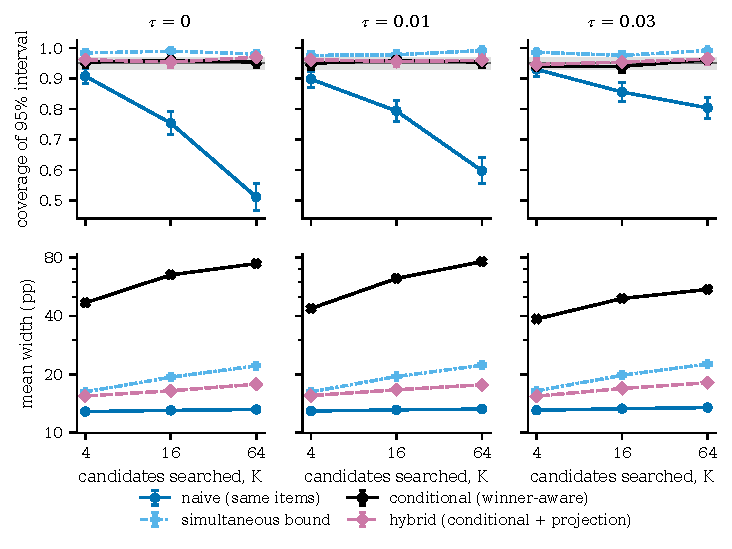
\includegraphics[width=\linewidth]{figures/e5b_hybrid_n200.pdf}
\caption{Winner-aware intervals for the argmax winner ($n=200$, $\rho=0.5$, $500$ repetitions). Coverage of the nominal 95\% interval for the true score of the selected configuration (bars $\pm1.96$ s.e.; grey band: binomial Monte-Carlo band) and mean width (log scale) for the naive, simultaneous, conditional and hybrid intervals.}\label{fig:hybrid}
\end{figure}


\begin{figure}[tbp]
\centering
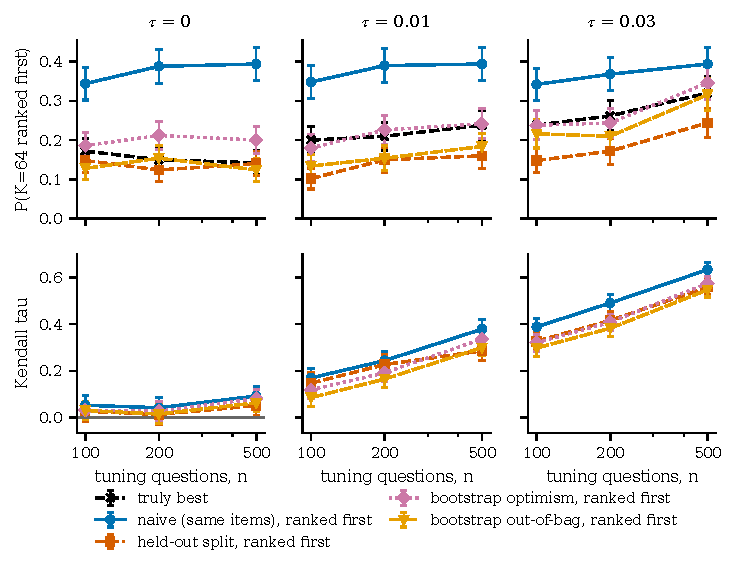
\includegraphics[width=\linewidth]{figures/e4c_ranking.pdf}
\caption{Ranking five systems tuned on the same items with $K=4,8,16,32,64$ configurations (best-of-$K$, $500$ repetitions). Top: share of repetitions in which each method ranks the $K=64$ system first, against how often it is truly best (black dashed). Bottom: mean Kendall's $\tau$ between reported and true ranking.}\label{fig:rank}
\end{figure}

\begin{figure}[tbp]
\centering
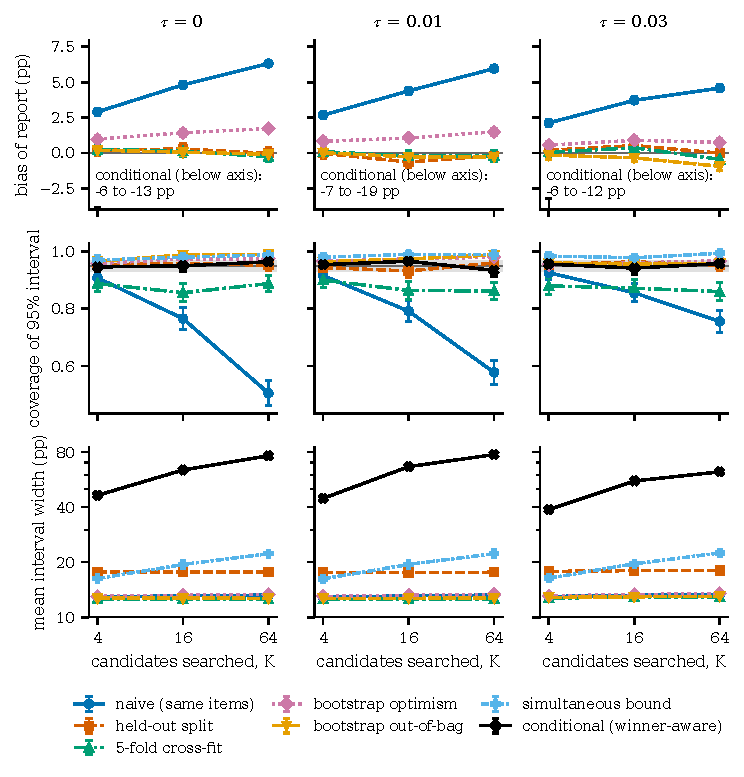
\includegraphics[width=\linewidth]{figures/e5_reliability_argmax_rho0.5_n200.pdf}
\caption{Reporting methods against the exact truth ($n=200$, $\rho=0.5$, best-of-$K$, $500$ repetitions). Top: bias of the reported score. Middle: coverage of the nominal 95\% interval (grey band: binomial 95\% Monte-Carlo band). Bottom: mean interval width (log scale). The conditional method lies below the plotted bias range (see panel text) and has intervals $40$--$80$~pp wide.}\label{fig:reliab}
\end{figure}

\section{Generator calibrated to the real matrix}\label{app:calib}
To check that the synthetic generator is informative about real tuned scores, we built generator settings that match the real matrix and compared their naive gap with the real replay (Table~\ref{tab:calib}). Both settings use the $\N{real_K}$ real accuracies as the configuration accuracies and as the thresholds of a Gaussian copula over items: (i) one common latent correlation, chosen ($\rho=\N{gen_rho}$) to reproduce the mean pairwise $\varphi$ of the real $0/1$ matrix; (ii) the full matrix of pairwise tetrachoric correlations of the real data ($\N{gen_clip}$ eigenvalues clipped to make it positive semi-definite). Each generator is run on $10$ pools of $2000$ items with $300$ repetitions each, with the replay procedure of the real study. Mean accuracy, the spread of accuracies, the dispersion of item difficulty (standard deviation across items of the share of configurations solving the item: $\N{gen_sditem_real}$ real, $\N{gen_sditem_gen}$ generator) and the mean $\varphi$ are matched by the one-$\rho$ copula (the pairwise copula shares the thresholds). The one-$\rho$ copula cannot reproduce the heterogeneity of the pairwise $\varphi$ (real $\N{gen_phi_min}$--$\N{gen_phi_max}$; largest pairwise error $\N{gen_pw_err_uni}$) and overstates the gap at $K\ge4$; the pairwise copula matches every pair (largest error $\N{gen_pw_err_tet}$) and understates it slightly, probably through higher-order structure that a Gaussian copula does not carry. At mean accuracy $0.195$, latent $\rho=0.3,0.5,0.7,0.9$ correspond to an observed $\varphi$ of $\N{phimap_3},\N{phimap_5},\N{phimap_7},\N{phimap_9}$; the real $\varphi=\N{gen_phi_real}$ lies between the grid values $\rho=0.5$ and $0.9$ of the synthetic study, and the grid's mean accuracy of $0.3$ instead of $0.18$ changes $\varphi$ at equal $\rho$ by about $0.03$ ($\N{phimap_m3_r5}$ vs.\ $\N{phimap_5}$ at $\rho=0.5$). Over all $\N{gen_uni_cells}$ cells ($K=1,\dots,\N{real_K}$, $n$ up to $\N{gm_nmax}$, both arms) the one-$\rho$ copula differs from the replay by more than two Monte-Carlo s.e. in $\N{gen_uni_z2}$ cells and the pairwise copula in $\N{gen_tet_z2}$.
\begin{table}[h]
\centering
\caption{Generator calibrated to the real matrix against the real replay.}\label{tab:calib}
{\footnotesize\setlength{\tabcolsep}{3.5pt}
\begin{tabular}{lrrr}
\toprule
quantity & real matrix & one-rho copula & pairwise copula \\
\midrule
accuracy, mean (\%) & 18.23 & 18.21 & (same thresholds) \\
accuracy, sd across configs (pp) & 1.16 & 1.17 & (same thresholds) \\
item difficulty, sd across items & 0.232 & 0.231 & -- \\
mean pairwise $\phi$ & 0.348 & 0.344 & -- \\
pairwise $\phi$, min--max & $-$0.007--0.926 & 0.321--0.366 & -- \\
pairwise $\phi$, max $|\Delta|$ over pairs & -- & 0.572 & 0.053 \\
\midrule
naive gap, $n$=200, $K$=2 (pp) & $1.09 \pm 0.09$ & $1.14 \pm 0.05$ (+0.5) & $1.09 \pm 0.05$ ($-$0.0) \\
naive gap, $n$=200, $K$=4 (pp) & $2.07 \pm 0.08$ & $2.04 \pm 0.05$ ($-$0.4) & $1.97 \pm 0.05$ ($-$1.1) \\
naive gap, $n$=200, $K$=8 (pp) & $2.81 \pm 0.08$ & $2.95 \pm 0.05$ (+1.5) & $2.67 \pm 0.05$ ($-$1.6) \\
naive gap, $n$=200, $K$=16 (pp) & $3.39 \pm 0.08$ & $3.57 \pm 0.04$ (+2.1) & $3.31 \pm 0.05$ ($-$0.9) \\
naive gap, $n$=200, $K$=32 (pp) & $3.81 \pm 0.08$ & $4.30 \pm 0.04$ (+5.6) & $3.83 \pm 0.05$ (+0.2) \\
naive gap, $n$=200, $K$=60 (pp) & $4.18 \pm 0.07$ & $4.85 \pm 0.04$ (+7.8) & $4.14 \pm 0.04$ ($-$0.4) \\
\midrule
generator $-$ real, mean ($K\ge4$, \%) & -- & $+6.8$ & $-1.3$ \\
generator $-$ real, range ($K\ge4$, \%) & -- & $-10$ to $+16$ & $-14$ to $+4$ \\
cells with $|z|>2$ & -- & 31 of 63 & 4 of 63 \\
\bottomrule
\end{tabular}}

\par\smallskip\begin{minipage}{.97\linewidth}\footnotesizeGaussian-copula generator calibrated to the real matrix (accuracies as thresholds): one common latent correlation (``one-rho'', matched to the mean pairwise $\phi$) or one per pair (``pairwise copula'', tetrachoric correlations, 19 eigenvalues clipped). Gap rows: disjoint truth arm, mean $\pm$ s.e. (pp) of the generator (10 pools $\times$ 300 replications) with $z$ against the real replay in parentheses. Summary rows pool all $n$ (50, 100, 200, 400, 800) and both truth arms (disjoint and iid). The copula cannot reproduce the heterogeneity of the real pairwise dependence (near-duplicate and near-independent pairs) and, for the pairwise version, higher-order structure.
\end{minipage}
\end{table}

\section{Real-LLM setup and compute record}\label{app:setup}
Table~\ref{tab:setup} records the model, data revision, scoring protocol and compute of the real-LLM study as read from the committed compute log.
\begin{table}[h]
\centering
\caption{Setup and compute record of the real-LLM study (read from the compute log).}\label{tab:setup}
{\footnotesize\setlength{\tabcolsep}{3.5pt}
\begin{tabular}{lp{0.64\linewidth}}
\toprule
item & value \\
\midrule
model & Qwen2.5-0.5B-Instruct, fp32, CPU; option-letter log-probabilities \\
benchmark & MMLU-Pro test, revision \texttt{b189ec765aa7}, 2000 questions (seed 2024) \\
configurations & 60 complete of 60 planned (instruction wording $\times$ demo set $\times$ layout) \\
forward passes & 120,000 scored of 120,000 planned \\
accuracy across configs & mean 18.2\%, range 15.2--20.8\%, sd 1.16 pp \\
item correlation & mean pairwise correlation of item correctness across configs 0.35 \\
scoring jobs & 10 scoring jobs of 6 configurations each, all finished; wall-clock 20.7--34.7 h per job (0.7 h for the job resumed after an out-of-memory stop) \\
replay jobs & real replay K=60 disjoint (argmax/sh/sr/greedy), M=1000 85 min; real replay K=60 iid, M=1000 109 min \\
seeds & configs/demos 12345, questions 2024, replay 5 \\
packages & Python 3.11.2, numpy 2.4.6, scipy 1.17.1, pandas 3.0.6, scikit-learn 1.9.1, torch 2.14.1+cpu, transformers 5.22.1 \\
\bottomrule
\end{tabular}}

\par\smallskip\begin{minipage}{.97\linewidth}\footnotesizeSetup and compute record of the real-LLM matrix, from the compute log and the matrix summary; all 60 planned configurations are scored. Scoring wall-clock is elapsed time in the job on a shared host and includes time the container was frozen, so it exceeds the CPU time used. Replay times are the logged running times.
\end{minipage}
\end{table}
